\section{Parallel histogram calculation using OpenMP \punkte{15}}

I looked into various synchronization strategies with OpenMP, creating three parallel versions of the histogram computation. There’s the \texttt{atomic} version, a \texttt{Merge Critical} version that merges everything within the parallel region, and then there’s the \texttt{Merge Out} version, which handles merging sequentially outside that region.

\subsection*{Implementation}

\lstinputlisting[
    language=C++,
    numbers=left,
    caption={Histogram with private histograms and in-region merge (Merge Critical)},
    captionpos=b,
    label={lst:mergeCritical},
    linerange={38-58},
    firstnumber=38
]{../Skeleton_codes/hist/hist_omp.cpp}

\lstinputlisting[
    language=C++,
    numbers=left,
    caption={Histogram with private histograms and external merge (Merge Out)},
    captionpos=b,
    label={lst:mergeOut},
    linerange={61-88},
    firstnumber=61
]{../Skeleton_codes/hist/hist_omp.cpp}

\lstinputlisting[
    language=C++,
    numbers=left,
    caption={Histogram with atomic updates},
    captionpos=b,
    label={lst:atomic},
    linerange={91-98},
    firstnumber=91
]{../Skeleton_codes/hist/hist_omp.cpp}

The \texttt{Merge Critical} version was created to allow a thread that finishes its task early to begin merging its partial results right away, even if the other threads are still working. On the flip side, in the \texttt{Merge Out} version, all the threads finish their heavy computation first before they go through a single merge process in sequence.

\subsection*{Performance analysis}
Figure~\ref{fig:histScaling} shows the impressive scaling results we got from the cluster. Up to about 16–20 physical cores, both versions scale pretty well, but the \texttt{Merge Out} version actually does a bit better overall. This seems to indicate that steering clear of synchronization during the parallel section leads to better efficiency, even if the merge step itself is all done sequentially at the end. The anticipated benefit of merging within the region earlier just didn’t pan out, probably because the costs of locking and competing for cache space outweighed any potential gains.

What’s surprising is that when we bumped up the thread count from 8 to 16 in the \texttt{Merge Critical} version, the runtime actually got worse, which doesn’t really make sense given that 20 cores were available. This is likely due to increased contention over the critical section lock along with the overheads from OpenMP’s runtime scheduling and synchronization.

It’s also worth mentioning that the \texttt{atomic} version didn’t perform well at any thread count, even falling short of the sequential baseline. This is mainly because of heavy contention and cache-line conflicts since each atomic increment pretty much serializes access to the shared histogram array.

\begin{figure}[H]
    \centering
    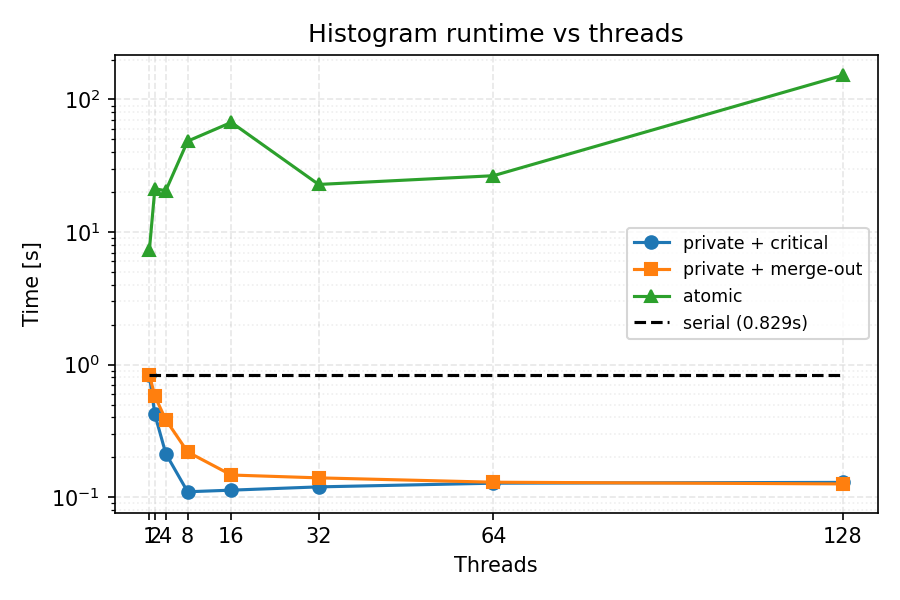
\includegraphics[width=0.8\textwidth]{../Skeleton_codes/hist/plots/hist_runtime_scaling.png}
    \caption{Strong scaling of the three OpenMP histogram versions.}
    \label{fig:histScaling}
\end{figure}

\noindent
The findings highlight that cutting down on synchronization in the parallel section is crucial for improving performance. Even though both merging methods work, the external merge (\texttt{Merge Out}) shows better scalability, whereas the \texttt{atomic} method isn't very efficient for this task.
